\documentclass[10pt]{article}
\usepackage[UTF8]{ctex}
\usepackage{picinpar,graphicx,bm}
\usepackage{booktabs}
\usepackage{diagbox}
\usepackage{subfigure}
\usepackage{float}
\usepackage{cases}
\usepackage{multirow}
\usepackage{algorithm}  
\usepackage{algorithmic}

\usepackage{listings}
\usepackage{xcolor}
% 定义可能使用到的颜色
\definecolor{CPPLight}  {HTML} {686868}
\definecolor{CPPSteel}  {HTML} {888888}
\definecolor{CPPDark}   {HTML} {262626}
\definecolor{CPPBlue}   {HTML} {4172A3}
\definecolor{CPPGreen}  {HTML} {487818}
\definecolor{CPPBrown}  {HTML} {A07040}
\definecolor{CPPRed}    {HTML} {AD4D3A}
\definecolor{CPPViolet} {HTML} {7040A0}
\definecolor{CPPGray}  {HTML} {B8B8B8}
\lstset{
    columns=fixed,    
   % numbers=left,                                        % 在左侧显示行号
    frame=none,                                          % 不显示背景边框
    backgroundcolor=\color[RGB]{245,245,244},            % 设定背景颜色
    keywordstyle=\color[RGB]{40,40,255},                 % 设定关键字颜色
    numberstyle=\footnotesize\color{darkgray},           % 设定行号格式
    commentstyle=\it\color[RGB]{0,96,96},                % 设置代码注释的格式
    stringstyle=\rmfamily\slshape\color[RGB]{128,0,0},   % 设置字符串格式
    showstringspaces=false,                              % 不显示字符串中的空格
    language=c++,                                        % 设置语言
    morekeywords={alignas,continute,friend,register,true,alignof,decltype,goto,
    reinterpret_cast,try,asm,defult,if,return,typedef,auto,delete,inline,short,
    typeid,bool,do,int,signed,typename,break,double,long,sizeof,union,case,
    dynamic_cast,mutable,static,unsigned,catch,else,namespace,static_assert,using,
    char,enum,new,static_cast,virtual,char16_t,char32_t,explict,noexcept,struct,
    void,export,nullptr,switch,volatile,class,extern,operator,template,wchar_t,
    const,false,private,this,while,constexpr,float,protected,thread_local,
    const_cast,for,public,throw,std,size_t,__global__,__device__,__host__},
    emph={map,set,multimap,multiset,unordered_map,unordered_set,
    unordered_multiset,unordered_multimap,vector,string,list,deque,
    array,stack,forwared_list,iostream,memory,shared_ptr,unique_ptr,
    random,bitset,ostream,istream,cout,cin,endl,move,default_random_engine,
    uniform_int_distribution,iterator,algorithm,functional,bing,numeric,},
    emphstyle=\color{CPPViolet}, 
    frame=shadowbox,
    basicstyle=\footnotesize\ttfamily,
    tabsize=4,
}

\newcommand{\tabincell}[2]{\begin{tabular}{@{}#1@{}}#2\end{tabular}}  


%layout
\usepackage{calc} 
\setlength\textwidth{7in} 
\setlength\textheight{9in} 
\setlength\oddsidemargin{(\paperwidth-\textwidth)/2 - 1in}
\setlength\topmargin{(\paperheight-\textheight -\headheight-\headsep-\footskip)/2 - 1.5in}


\title{计算机图形学 \hspace{2pt}\hspace{2pt} \begin{large}----- \hspace{2pt} 蒙特卡罗光线跟踪算法 \end{large} }
\author{11821095 葛林林}
\begin{document}
\maketitle
\section{预备知识}
\subsection{光照模型}
\begin{itemize}
\item[(1)]{\bm{环境光}}:环境光无处不在,无论表面的法向如何,明暗程度都是一致的。
\item[(2)]{\bm{点光源}}:光源来自某个点,且向四面八方辐射。
\item[(3)]{\bm{平行光}}:又称为镜面光,这种光是互相平行的。从手电筒或者太阳出来的光都可以被看做平行光。
\item[(4)]{\bm{聚光灯}}:这种光源的光线从一个锥体中射出,在被照射的物体上产生聚光的效果。使用这种光源需要指定光的射出方向以及锥体的顶角$\alpha$。
\end{itemize}
\subsubsection{Lambertian光照模型(漫反射效果的仿真)}

\subsubsection{BlinnPhong光照模型(镜面反射效果的仿真)}
\begin{itemize}
\item[(1)]{\bm{发射光}} \mbox{}\\
$$C_{e}=M_{e}$$
$C_e$:发射颜色 \\
$M_e$:发射材质颜色

\item[(2)]{\bm{漫反射}} \mbox{}\\
定义漫反射因子$\alpha$如下:
$$\alpha=max\{0,N \cdot L\}$$
其中$L$是光线,$N$是定点法线向量。
$$C_{d}=L_{d}M_{d}\alpha$$
\end{itemize}


\subsection{obj文件介绍}
obj文件并不考虑物体的大小,所以不同的物体读入的坐标范围可能变化很大,因此为了显示的方便需将其转为当前绘制坐标系中。
\begin{itemize}
\item[(1)]{库相关}
\begin{itemize}
\item[•]{$\bm{mtllib}$ xxx} \mbox{} \\
材料库。
\item[•]{$\bm{usemtl}$ xxx} \mbox{} \\
代表使用xxx类型的材质。
\end{itemize}

\item[(2)]{组相关} 
\begin{itemize}
\item[•]{$\bm{g}$ xxx} \mbox{} \\
表示组,将xxx标签之后的多边形组成一个整体。
\item[•]{$\bm{s}$ xxx} \mbox{} \\
光滑组:加入光滑组之后能够让在同一组的多边形之间连接更为光滑,其中“s off”代表关闭光滑组。
\end{itemize}

\item[(3)]{坐标相关}
\begin{itemize}
\item[•]{$\bm{vt} \hspace{5pt}tu \hspace{5pt} tv$} \mbox{} \\
代表纹理坐标。
\item[•]{$\bm{vn} \hspace{5pt} nx \hspace{5pt} ny \hspace{5pt} nz$} \mbox{} \\
法向量的表示。
\item[•]{$\bm{f} \hspace{5pt} v/vt/vn \hspace{5pt} v/vt/vn \hspace{5pt} v/vt/vn$}\mbox{} \\
表示多边形,格式为“f 顶点索引 / 纹理坐标索引 / 顶点法向量索引”。
\item[•]{$\bm{v} \hspace{5pt} x\hspace{5pt}y\hspace{5pt}z$} \mbox{} \\
顶点以$v$开头后面跟着该顶点的$x,y,z$三轴坐标。
\end{itemize}

\end{itemize}

\subsection{mtl文件介绍}
mtl文件是用来描述文件材质的一个文件,描述的是物体的材质信息,ASCII存储,任何文本编辑器可以将其打开和编辑。一个.mtl文件可以包含一个或多个材质定义,对于每个材质都有其颜色,纹理和反射贴图的描述,应用于物体的表面和顶点。描述的是物体的材质信息,ASCII存储,任何文本编辑器可以将其打开和编辑。一个.mtl文件可以包含一个或多个材质定义,对于每个材质都有其颜色,纹理和反射贴图的描述,应用于物体的表面和顶点。:
\begin{itemize}
\item[(1)]{\bm{格式}:\bm{$Ka} \hspace{10pt} r \hspace{10pt} g \hspace{10pt} b$} \\
\bm{示例}:$\bm{Ks} \hspace{10pt} 0.588 \hspace{10pt} 0.588 \hspace{10pt} 0.588$\\
\bm{描述}:环境反射,用RGB颜色值来表示,g和b两参数是可选的,如果只指定了r的值,则g和b的值都等于r的值。三个参数一般取值范围为[0.0,1.0],在此范围外的值则相应的增加或减少反射率;

\item[(2)]{\bm{格式}:\bm{$Kd} \hspace{10pt} r \hspace{10pt} g \hspace{10pt} b$}\\
\bm{示例}:$\bm{Kd} \hspace{10pt} 0.65 \hspace{10pt} 0.65 \hspace{10pt} 0.65$\\
\bm{描述}:漫反射,$r g b$代表了RGB值,范围为[0,1]。其中$g$和$b$是可选的,如果未设置这两个值,则$g,b$的值与$r$的值相同。

\item[(3)]{\bm{格式}:\bm{$Ks} \hspace{10pt} r \hspace{10pt} g \hspace{10pt} b$}\\
\bm{示例}:$\bm{Ks} \hspace{10pt} 0.65 \hspace{10pt} 0.65 \hspace{10pt} 0.65$\\
\bm{描述}:镜面反射,$r g b$代表了RGB值,范围为[0,1]。其中$g$和$b$是可选的,如果未设置这两个值,则$g,b$的值与$r$的值相同。


\item[(4)]{\bm{格式}:\bm{$Tf} \hspace{10pt} r \hspace{10pt} g \hspace{10pt} b$}\\
\bm{示例}:$\bm{Tf} \hspace{10pt} 0.65 \hspace{10pt} 0.65 \hspace{10pt} 0.65$\\
\bm{描述}:代表了透射滤波,任何光线穿透该物体时可以利用该参数进行透射滤波,该参数只让指定颜色的光线穿透物体。例如Tf 0 1 0,只允许所有的绿色光线穿透,而所有的红色和绿色光线则不能够穿透。$r g b$代表了RGB值,范围为[0,1]。其中$g$和$b$是可选的,如果未设置这两个值,则$g,b$的值与$r$的值相同。

\item[(5)]{\bm{格式}:\bm{$illum} \hspace{10pt} number$} \\
\bm{示例}:\bm{$illum} \hspace{10pt} 2$\\
\bm{描述}:指定了光照模型。

\item[(6)]{\bm{$Ns \hspace{10pt} 10.000000$}}\\
指定材质的反射指数,定义了反射高光度。 exponent是反射指数值,该值越高则高光越密集,一般取值范围在$[0,1000]$。 

\item[(7)]{\bm{$Ni \hspace{10pt} 1.500000$}} \\
指定材质表面的光密度(即折射值),取值范围为$[0.001,10]$。若取值为1.0则光在通过物体的时候不发生弯曲。玻璃的折射率为1.5。取值小于1.0的时候可能会产生奇怪的结果不推荐。

\item[(8)]{\bm{$d \hspace{10pt} 1.000000$}}\\
表示物体融入背景的数量,取值范围为$[0.0,1.0]$,取值为1.0表示完全不透明,取值为0.0时表示完全透明。
\end{itemize}
\subsection{空间包围盒的介绍}
空间包围盒是一个物体的凸包,是为了物体与光线求交的方便而引入的概念。人们提出了很多种可用的空间包围盒,其中AABB包围盒最为简单和常用。AABB包围盒的所有边与坐标轴平行,其示意图如下所示,起哄蓝色的为物体,绿色表示的时该物体的AABB包围盒:
\begin{figure}[H]
\begin{center}
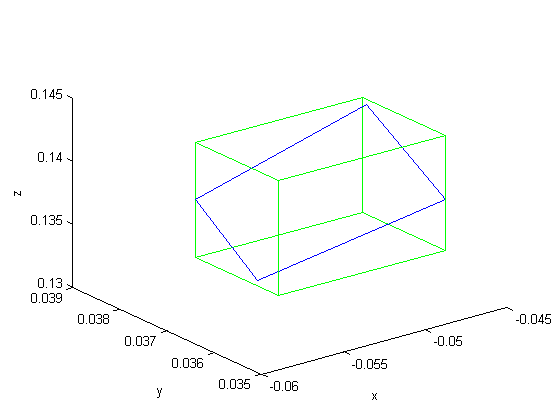
\includegraphics[scale=0.5]{AABB1.png}
\caption{AABB包围盒示意图}
\end{center}
\end{figure}
\subsection{Kd-Tree的介绍}
Kd-tree(K-dimension tree)是一种拥有多维空间的快速最近邻查找技术,它是一种将BST扩展到多维的升级。在使用Kd-tree的过程中极其重要的两个操作是创建和查找。
\subsubsection{Kd-Tree的构造}
\begin{itemize}
\item[(1)]{\bm{划分维度的选择}} \mbox{} \\
kd-tree在举例时都会按照第一维、第二维、第三维的循环顺序进行构建,然而在实际使用当中最主要的目的是加速,也就是尽快减少检索范围。每一层使用更为分散的维度能够更好的将数据进行分离。最大方差法就是利用方差最大的维度对数据进行划分。
\item[(2)]{\bm{构造截止条件}} \mbox{} \\
kd-tree在构造时满足一下任意条件则截止:
\begin{itemize}
\item{在该空间已经不存在数据点;}
\item{超过一定的深度则划定为叶子节点,该深度的阈值可以由自己来规定。}
\end{itemize}

\begin{figure}[H]
\begin{center}
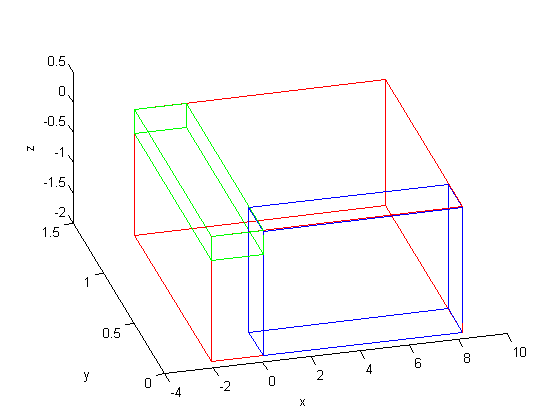
\includegraphics[scale=0.5]{kd-tree-structure.png}
\caption{kd-tree第一层和第二层示意图}
\end{center}
\end{figure}
\end{itemize}
\subsubsection{Kd-Tree的最近表面搜索策略}
本文中用到的最近表面的搜索策略是在广度优先搜索的基础上,分层的进行搜索,其伪代码如下所示:
\begin{algorithm}[H]
	\caption{Nearest Surface Search by Level}%算法标题
	\begin{algorithmic}[1]%一行一个标行号
		\STATE $B_s =$ Get current buffer size
		\FOR{$i =$ 0 to $B_s$}
		\IF{ It is leaf node }
		\IF{ This node is more close }
		\STATE Store this node
		\ENDIF		
		\ELSE
		\STATE Insert two children
		\ENDIF
		\STATE Remove this first $B_s$ number of node
		\ENDFOR
	\end{algorithmic}
\end{algorithm}



\subsection{相机光线的产生}
由于从相机出发逆向跟踪光路能够避免计算无法被看到的部分,从而大大降低计算量。下面介绍了如何从相机出发产生初始的逆向光线。假设相机的位置为$\bm{P}_{camera}$,Lookat的位置为$\bm{T}_0$,up的单位方向为$D_{up}$,则相机的单位前向方向$\bm{D}_{forward}$为:
$$\bm{D}_{forward}=\frac{\bm{T}_0-\bm{P}_{camera}}{||\bm{T}_0-\bm{P}_{camera}||}$$
除此之外,实际过程中所给的up方向并不是实际的相机朝上方向,如下图所示Supplied 'up' vector一般是所给的方向,而我们要去计算实际的Actual 'up' vector:
\begin{figure}[H]
\begin{center}
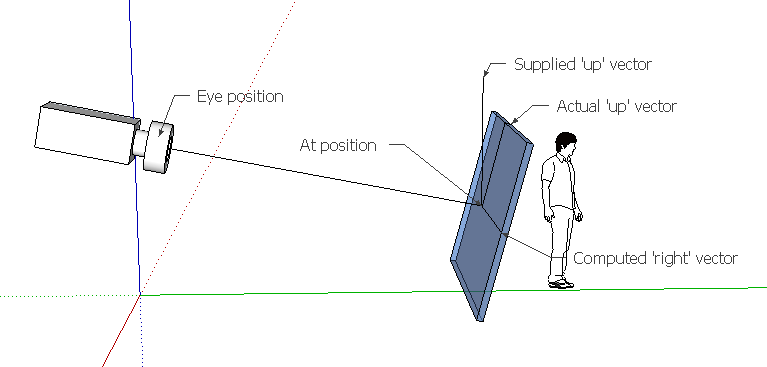
\includegraphics[scale=0.4]{up_adjust.png}
\caption{up方向的修正示意图}
\end{center}
\end{figure}
计算公式如下所示,注意保证$\bm{D}_{up}$和$\bm{D}_{forward}$保证是单位向量:
$$\theta=acos(\bm{D}_{up} \cdot \bm{D}_{forward})$$
则真正的$\bm{D}_{up}$可以有如下公式算出:
$$
\bm{D}_{up}=\left\{
\begin{array}{rl}
\bm{D}_{up}cos(\theta) \hspace{10pt} \theta >0 \\
-\bm{D}_{up}cos(\theta) \hspace{10pt} \theta \leq 0
\end{array}
\right.
$$
则指向像平面右侧的单位方向为$\bm{D}_{right}$:
$$\bm{D}_{right}=\bm{D}_{forward} \times \bm{D}_{up}$$
假设单个像素的实际宽度为$W$,宽度像素的实际个数为$N_{w}$,单个像素的实际高度为$H$,高度方向是像素个数为$N_{h}$,相机的焦距为$L$,则像平面左上角像素在世界坐标系下的位置$P_{0,0}$为:
$$P_{0,0}=\bm{P}_{camera}+L\bm{D}_{forward}-N_{w}WD_{right}+N_{h}HD_{up}$$

\subsection{求交检测}
\subsubsection{AABB包围盒与光线求交检测}

\subsubsection{凸多边形与光线求交检测}
判断光线与凸多边形求交检测的步骤如下:
\begin{itemize}
\item[(1)]{\bm{求取方程}} \mbox{} \\
求取凸多边形对应的平面方程和光线所在直线方程,假设平面方程为:
$$Ax+By+Cz+D=0$$
直线方程为:
$$
\left\{
\begin{array}{rl}
x=a_1t+b_1\\
y=a_2t+b_2\\
z=a_3t+b_3
\end{array}
\right.
$$
\item[(2)]{\bm{求取交点}} \mbox{} \\
计算凸多边形所在平面和光线所在直线方程的交点
\item[(3)]{\bm{判断方向是否一致}} \mbox{} \\
需要判断从光线原点出发到交点的射线方向是否与光线方向一致,假设光线原点为$\bm{r}_o$,光线方向为$\bm{r}_d$,交点坐标为$\bm{I}$,则有如下结论:
$$
\bm{r}_d(\bm{I}-\bm{r}_o)=
\left\{
\begin{array}{rl}
<0 & \hspace{20pt} no \hspace{10pt} intersection \\
>0 & \hspace{20pt} not \hspace{10pt} sure
\end{array}
\right.
$$
\item[(4)]{\bm{判断点和凸多边形关系}}  \mbox{} \\
如下图所示是交点与凸多边形的关系示意图
\begin{figure}[H]
\begin{center}
\subfigure[内部]{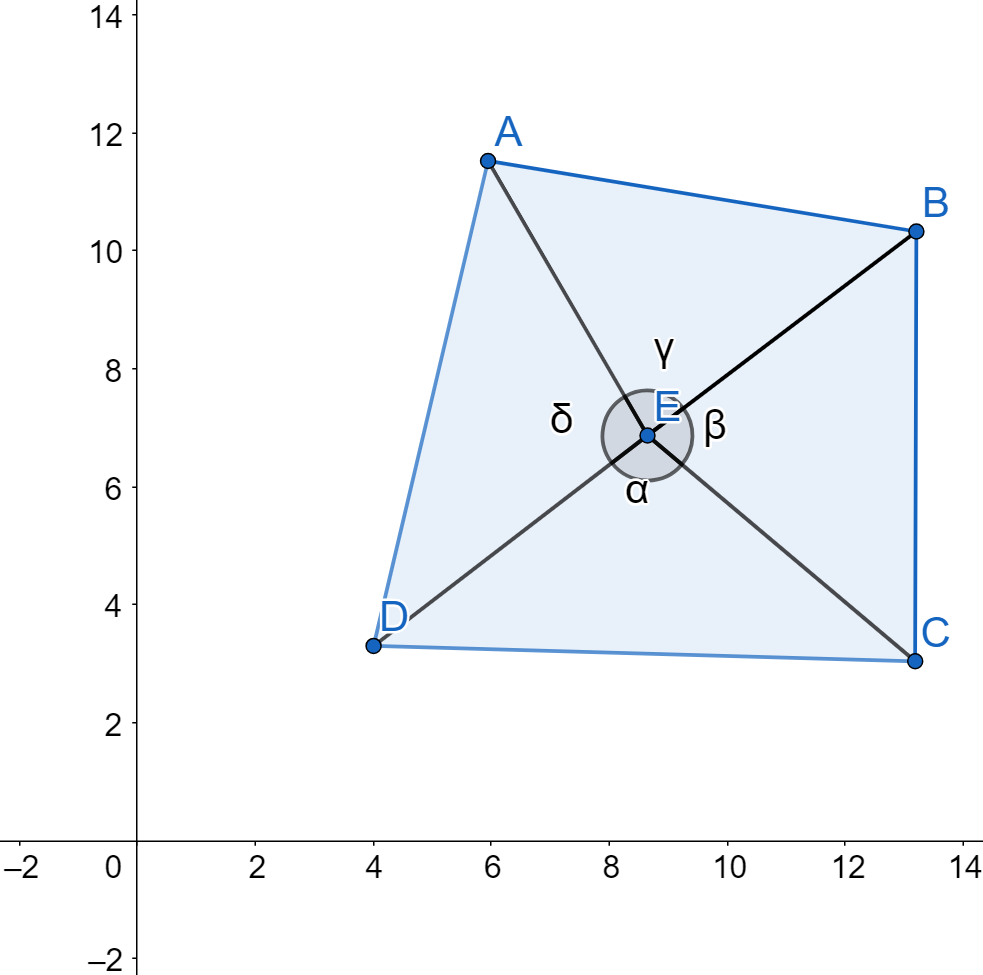
\includegraphics[scale=0.35]{case1.png}}
\hspace{20pt}
\subfigure[外部]{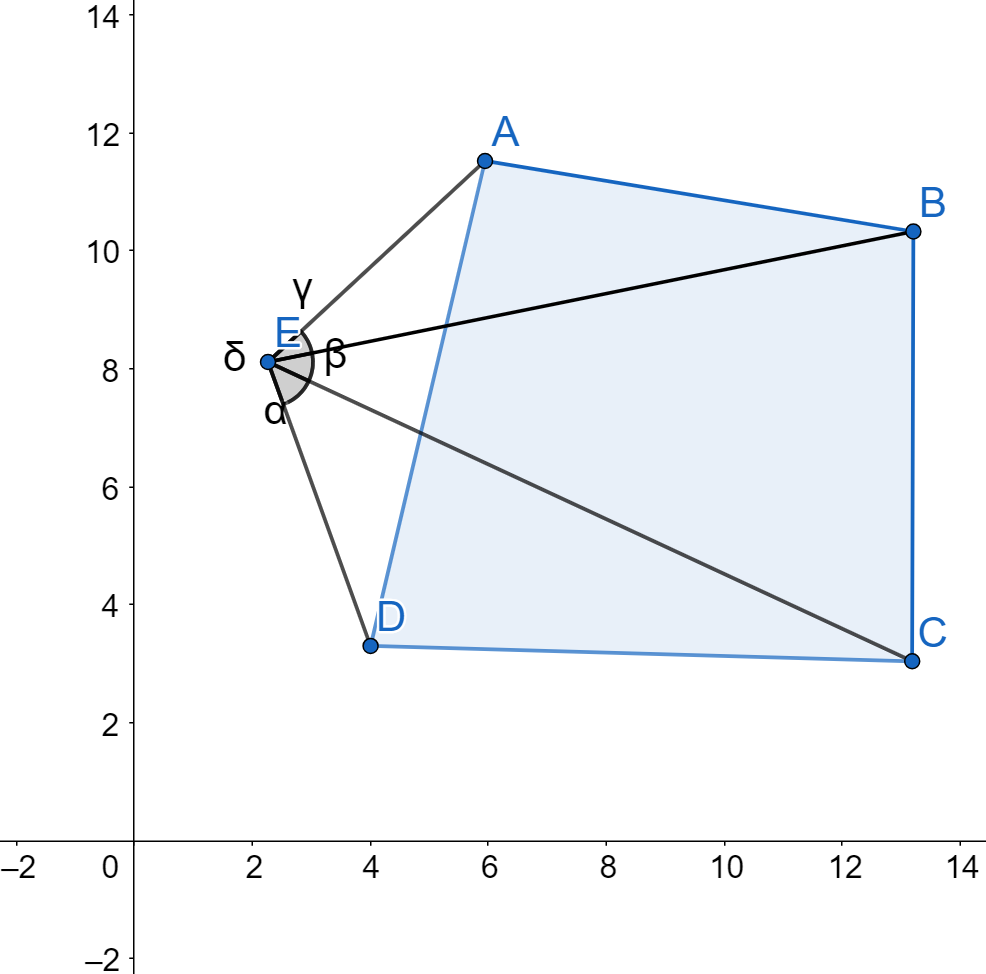
\includegraphics[scale=0.35]{case2.png}}
\caption{交点与凸多边形关系图}
\end{center}
\end{figure}
\end{itemize}
从上图中可以看出,内部的情况需要满足如下公式:
$$\alpha+\beta+\gamma+\sigma=2\pi$$
当在外部的情况下满足如下关系:
$$\alpha+\beta+\gamma+\sigma < 2\pi$$

\subsection{光线和球求交}
如下图所示是光线和球求交的示意图:
\begin{figure}[H]
\begin{center}
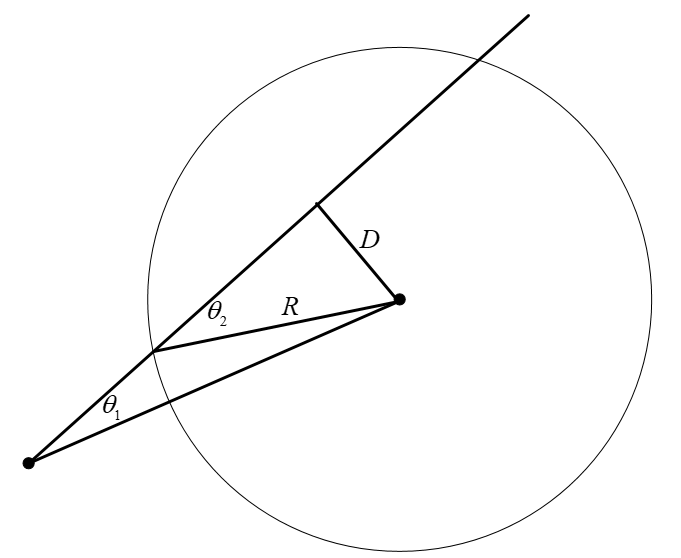
\includegraphics[scale=0.6]{intersection_ray_sphere.png}
\caption{光线和球求交检测示意图}
\end{center}
\end{figure}
则图中得到$L$的公式为:
$$\theta_1=arcsin(\frac{D}{L_1})$$
$$\theta_2=arsin(\frac{D}{R})$$
$$L_2=\frac{D}{tan(\theta_1)}-\frac{D}{tan(\theta_2)}$$

\section{步骤}
如下图所示是整个光线跟踪算法的处理流程图:
\begin{figure}[H]
\begin{center}
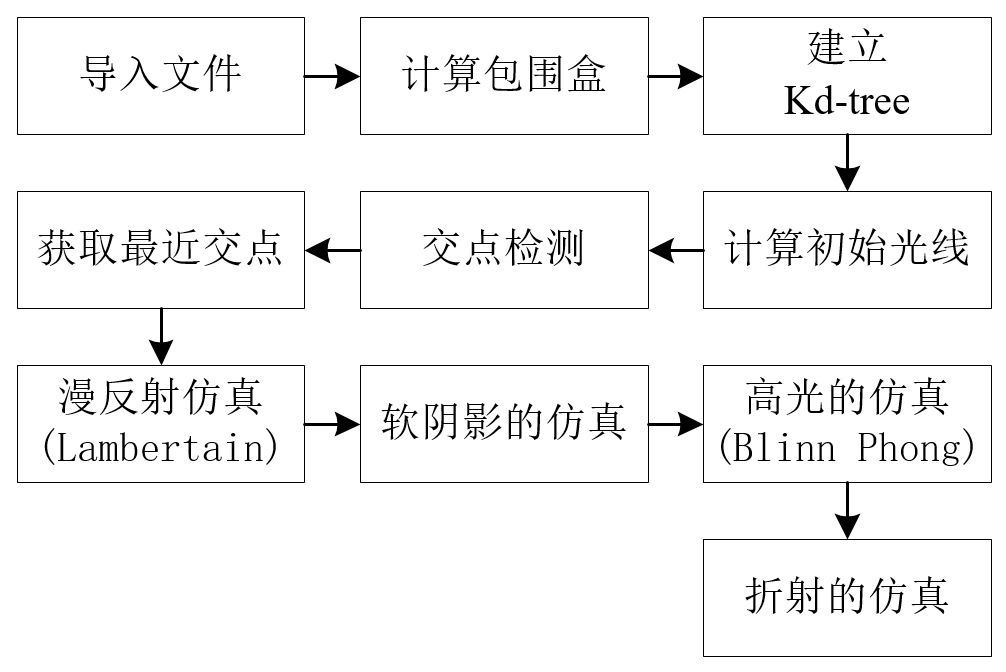
\includegraphics[scale=0.3]{chart_flow.png}
\caption{整体流程图}
\end{center}
\end{figure}

\section{实验结果}
\begin{figure}[H]
\begin{center}
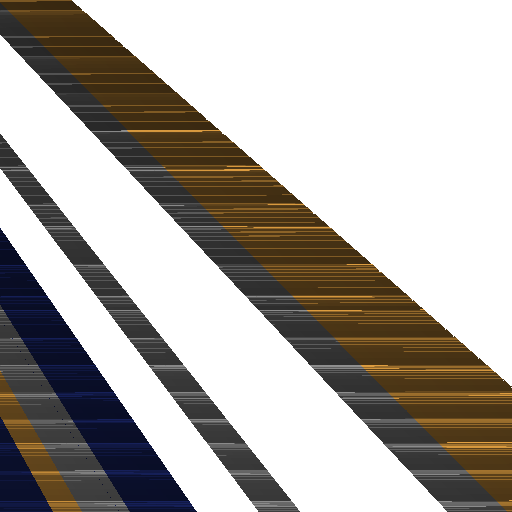
\includegraphics[scale=0.5]{result1.png}
\end{center}
\caption{Lambertian仿真漫反射的场景1效果图}
\end{figure}

\begin{figure}[H]
\begin{center}
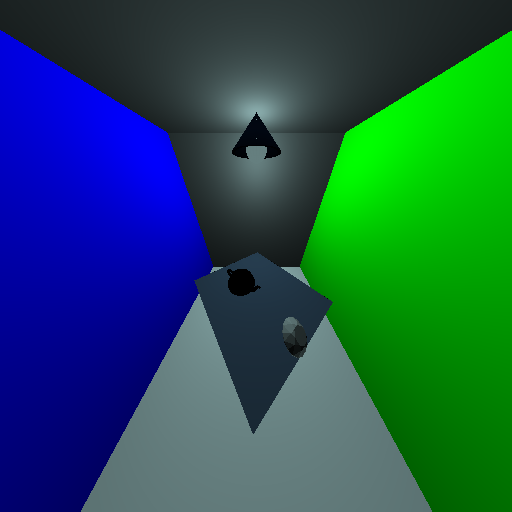
\includegraphics[scale=0.5]{result2.png}
\end{center}
\caption{Lambertian仿真漫反射的场景2效果图}
\end{figure}

\begin{figure}[H]
\begin{center}
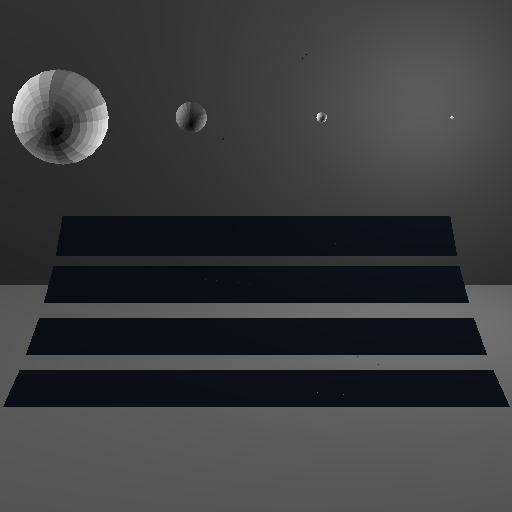
\includegraphics[scale=0.5]{result3.png}
\end{center}
\caption{Lambertian仿真漫反射的场景3效果图}
\end{figure}

\section{问题汇总}
\subsection{关于光线的疑问}
问题描述:在编程时光线如何存储?
光线的数学表达如下所示:
$$\bm{R}(t)=\bm{O}+t\bm{D}$$
其中$\bm{O}$为原点,$\bm{D}$为光线的方向(默认为单位向量),而$t$为距离。
\subsection{光照信息的存储}

\subsection{蒙特卡洛用在哪里?}
光线跟踪的交叉点的光照值通过RDBF模型来计算,RDBF模型中假设了采样点的光度值都是由来自各个方向的半球光线汇集得到的RGB值,如下图所示:
\begin{figure}[H]
\begin{center}
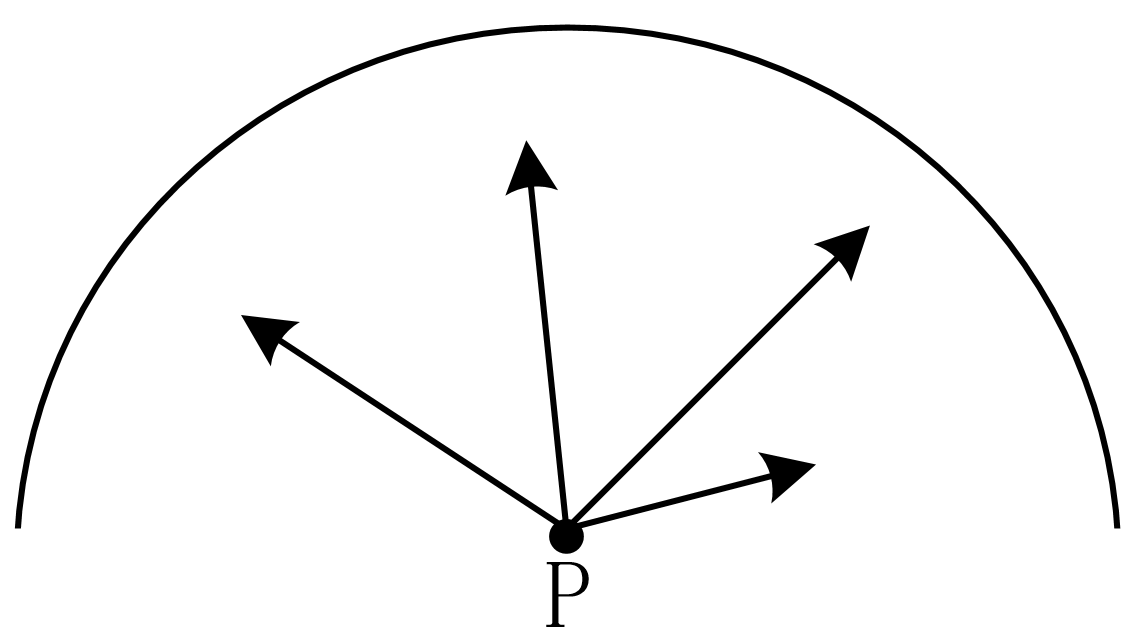
\includegraphics[scale=0.25]{monte_carlo_sample.png}
\caption{蒙特卡洛采样示意图}
\end{center}
\end{figure}
由于来自该半球方向的光线理论上有无线多条,因此采用蒙特卡洛方法随机的对方向进行采样。蒙特卡洛的结果可以看成是该半球光线积分的估计值。
\subsection{Kd-tree面对三角片如何构建?}
由于kd-tree分割的对象是点坐标,因此对于三角片可以用其中点代替三角片本身的位置,这样就可以很方便的确定kd-tree中心轴的位置。
\subsection{Kd-tree是如何与包围盒结合使用的?}
kd-tree的每一个节点都包含一个包围盒,该包围盒包括了该节点下的所有子节点空间。



\end{document}
